\section{Choice of screening threshold \label{App.thresholds}}

The figures below show the model performance, when using other screening thresholds.

\begin{center}
\begin{figure}[h]
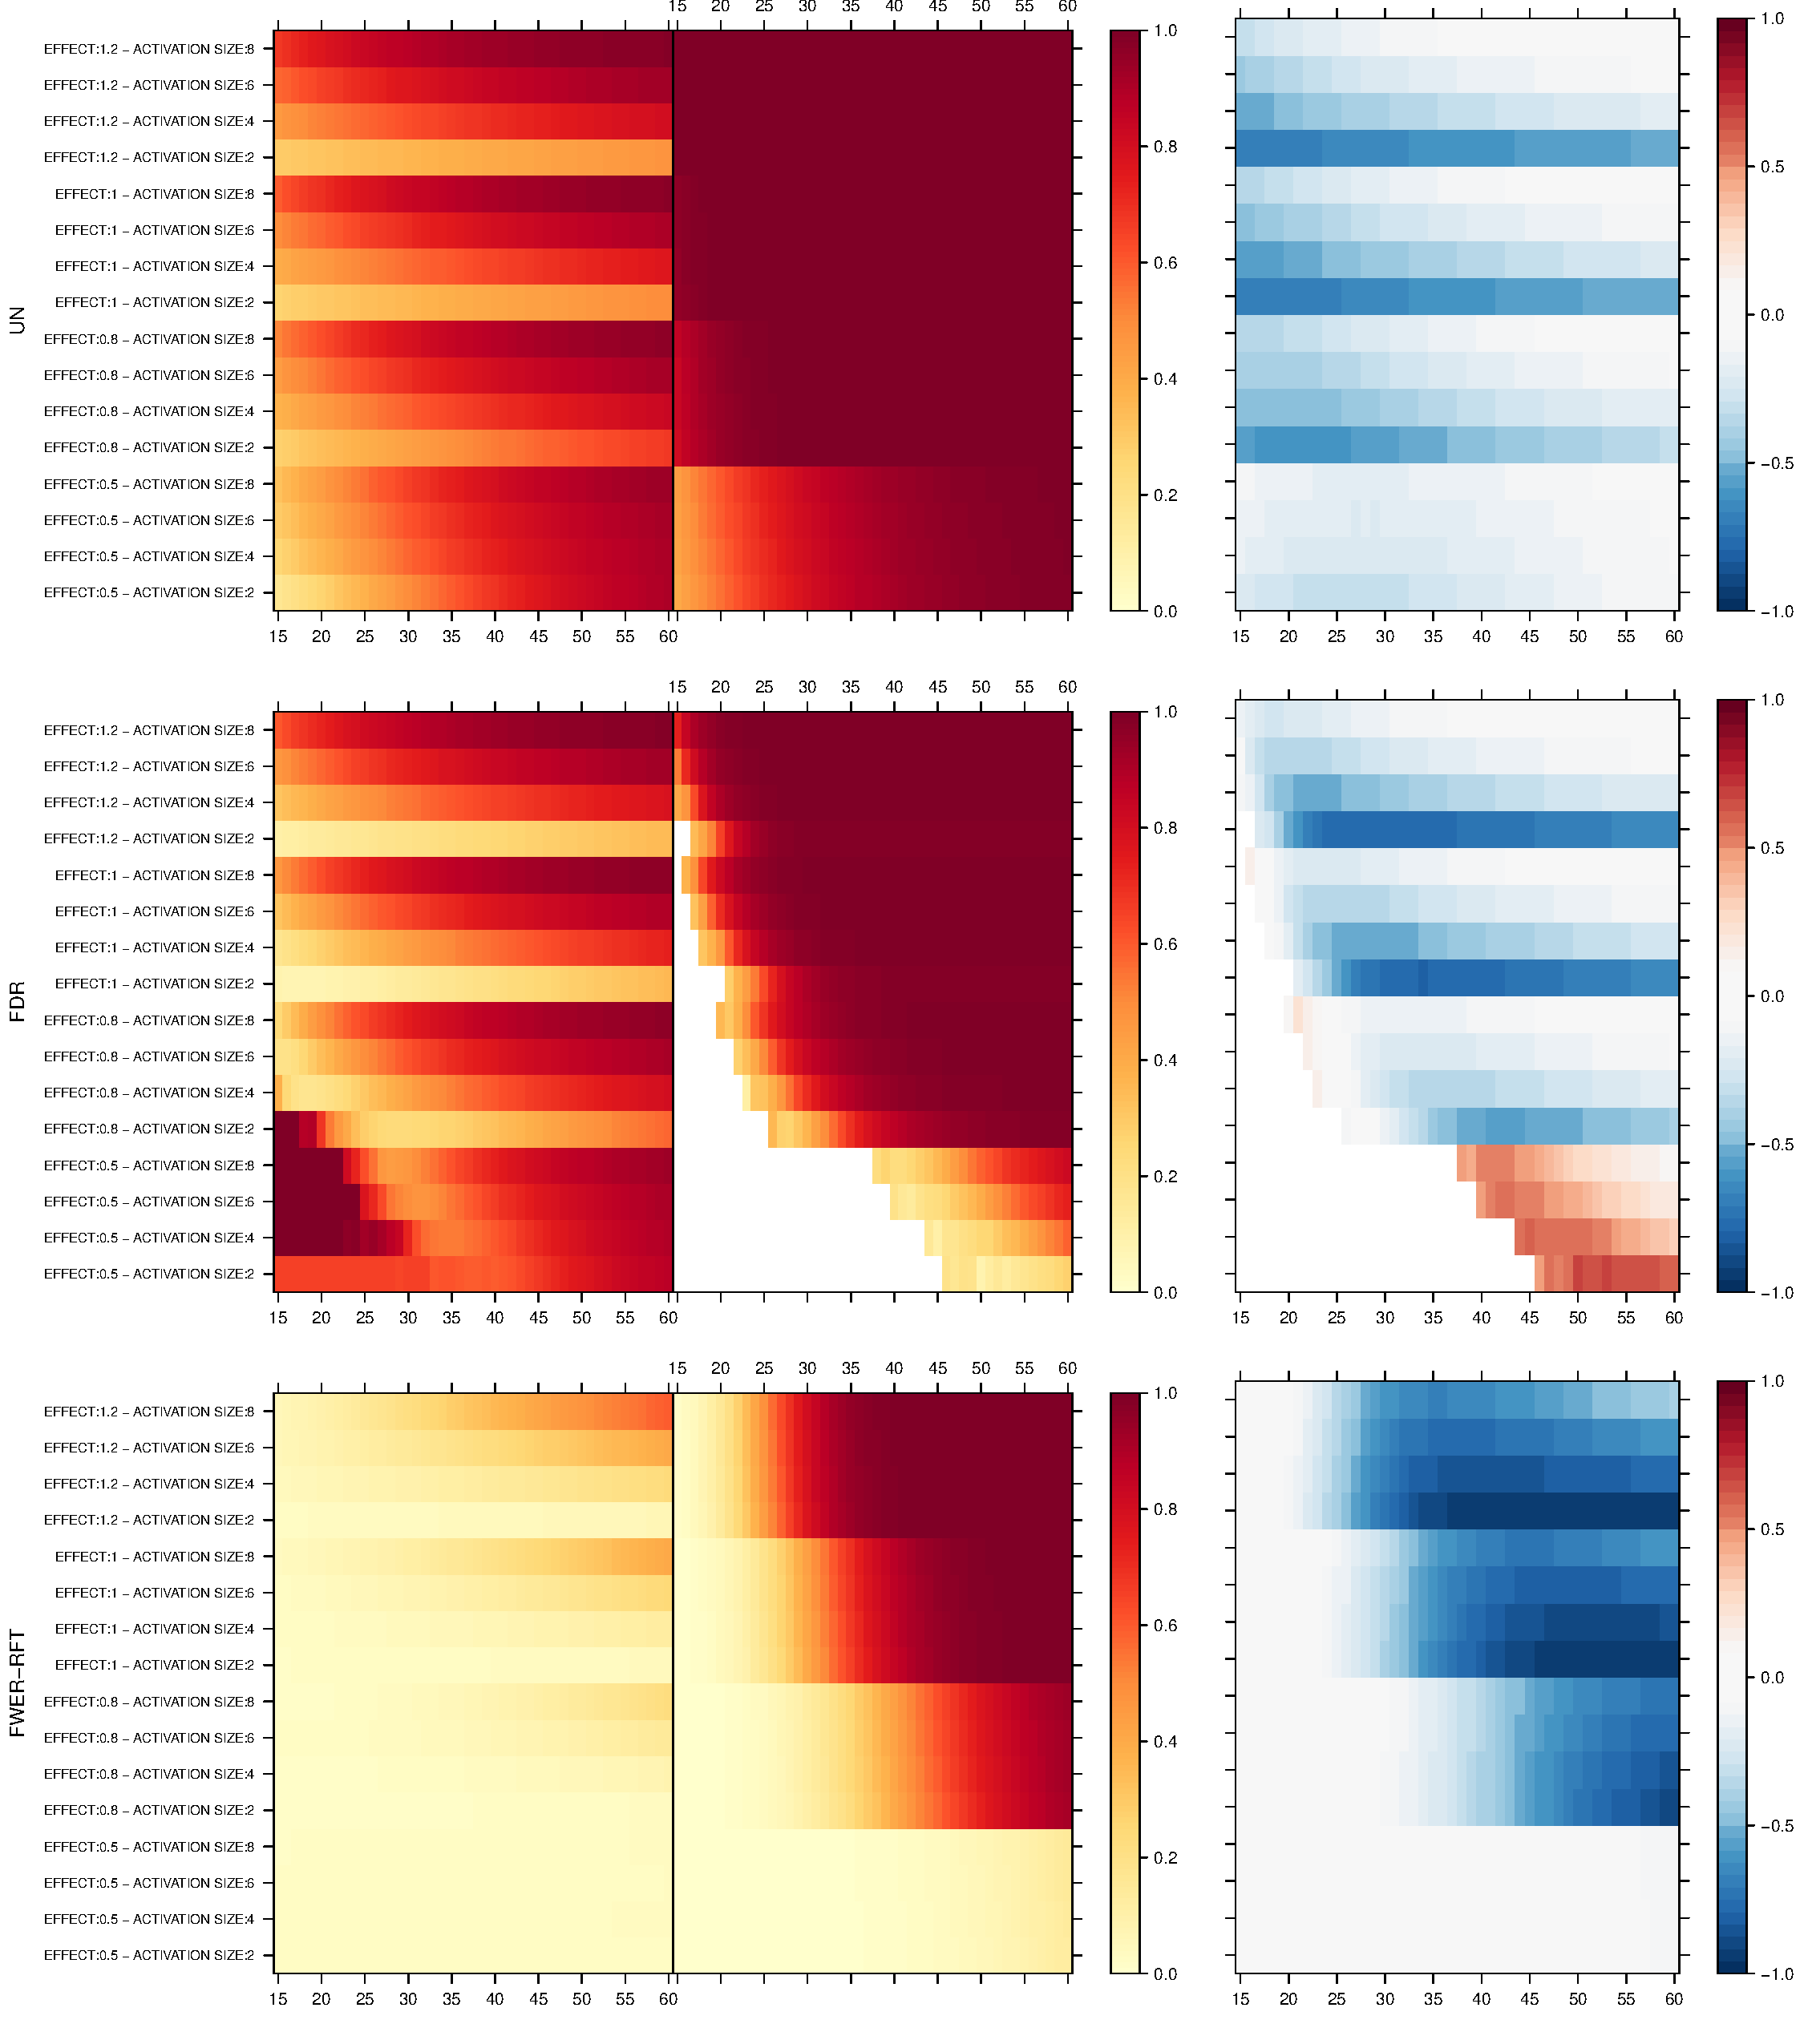
\includegraphics[scale=0.25]{figures/FIG_SIM_power_15_NOMASK_2_0.pdf}
\caption{Plots of the peakwise average power with error rate control at 5\% for different effect sizes and different amounts of activation, when using a screening threshold at 2.0.}
\end{figure}
\end{center}


\begin{center}
\begin{figure}[h]
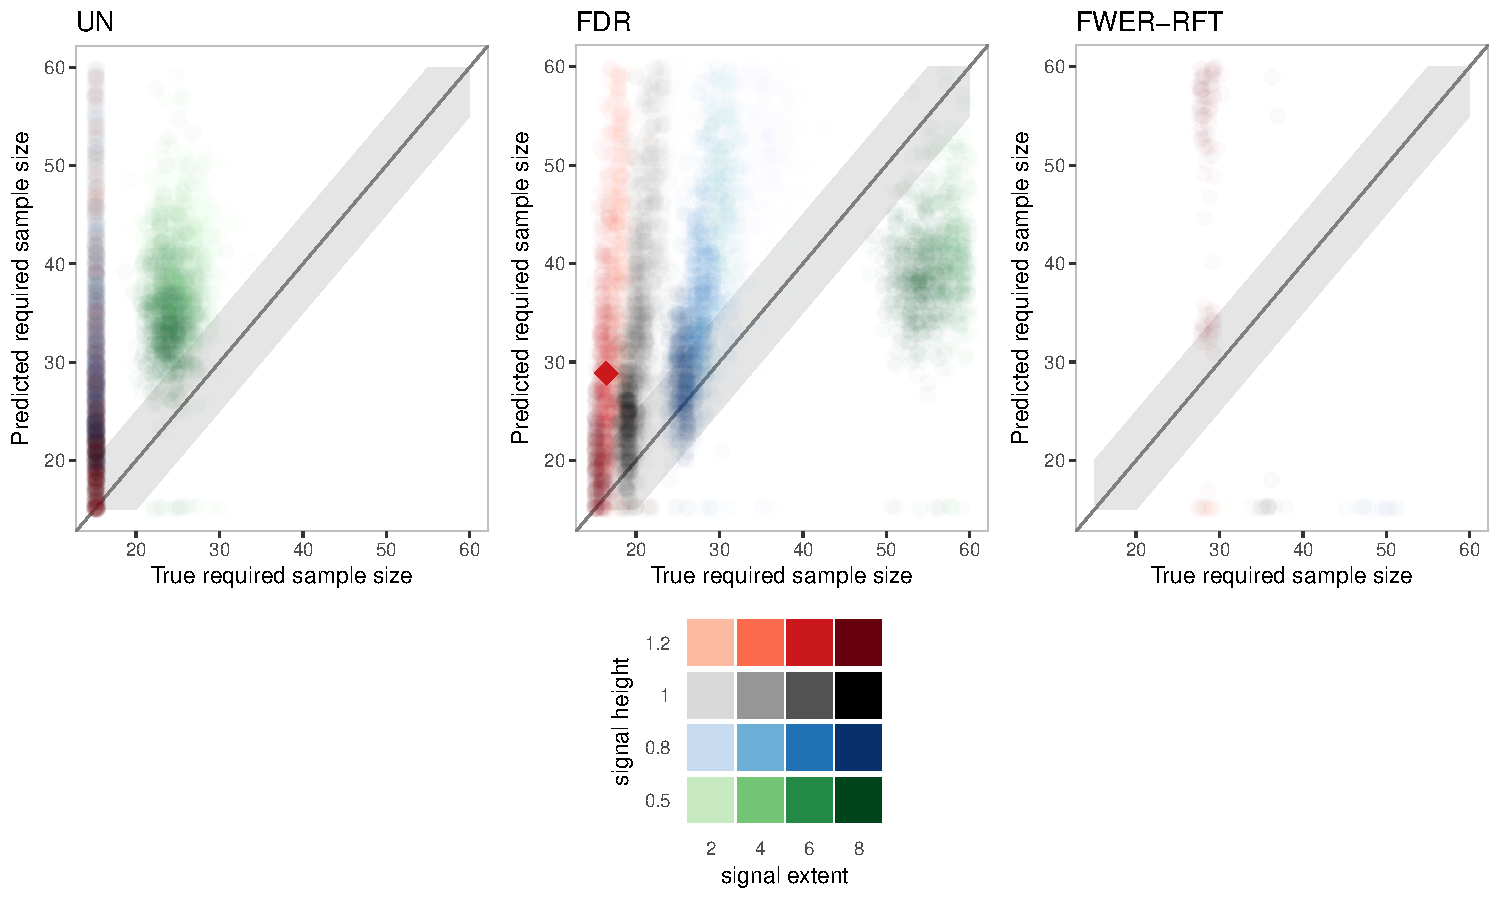
\includegraphics[scale=0.35]{figures/FIG_SIM_sscalc_15_NOMASK_2_0.pdf}
\caption{Plots of the predicted and true required sample size when 80\% power is desired. The different plots refer to the different multiple testing procedures, when using a screening threshold at 2.0.}
\end{figure}
\end{center}

\begin{center}
\begin{figure}[h]
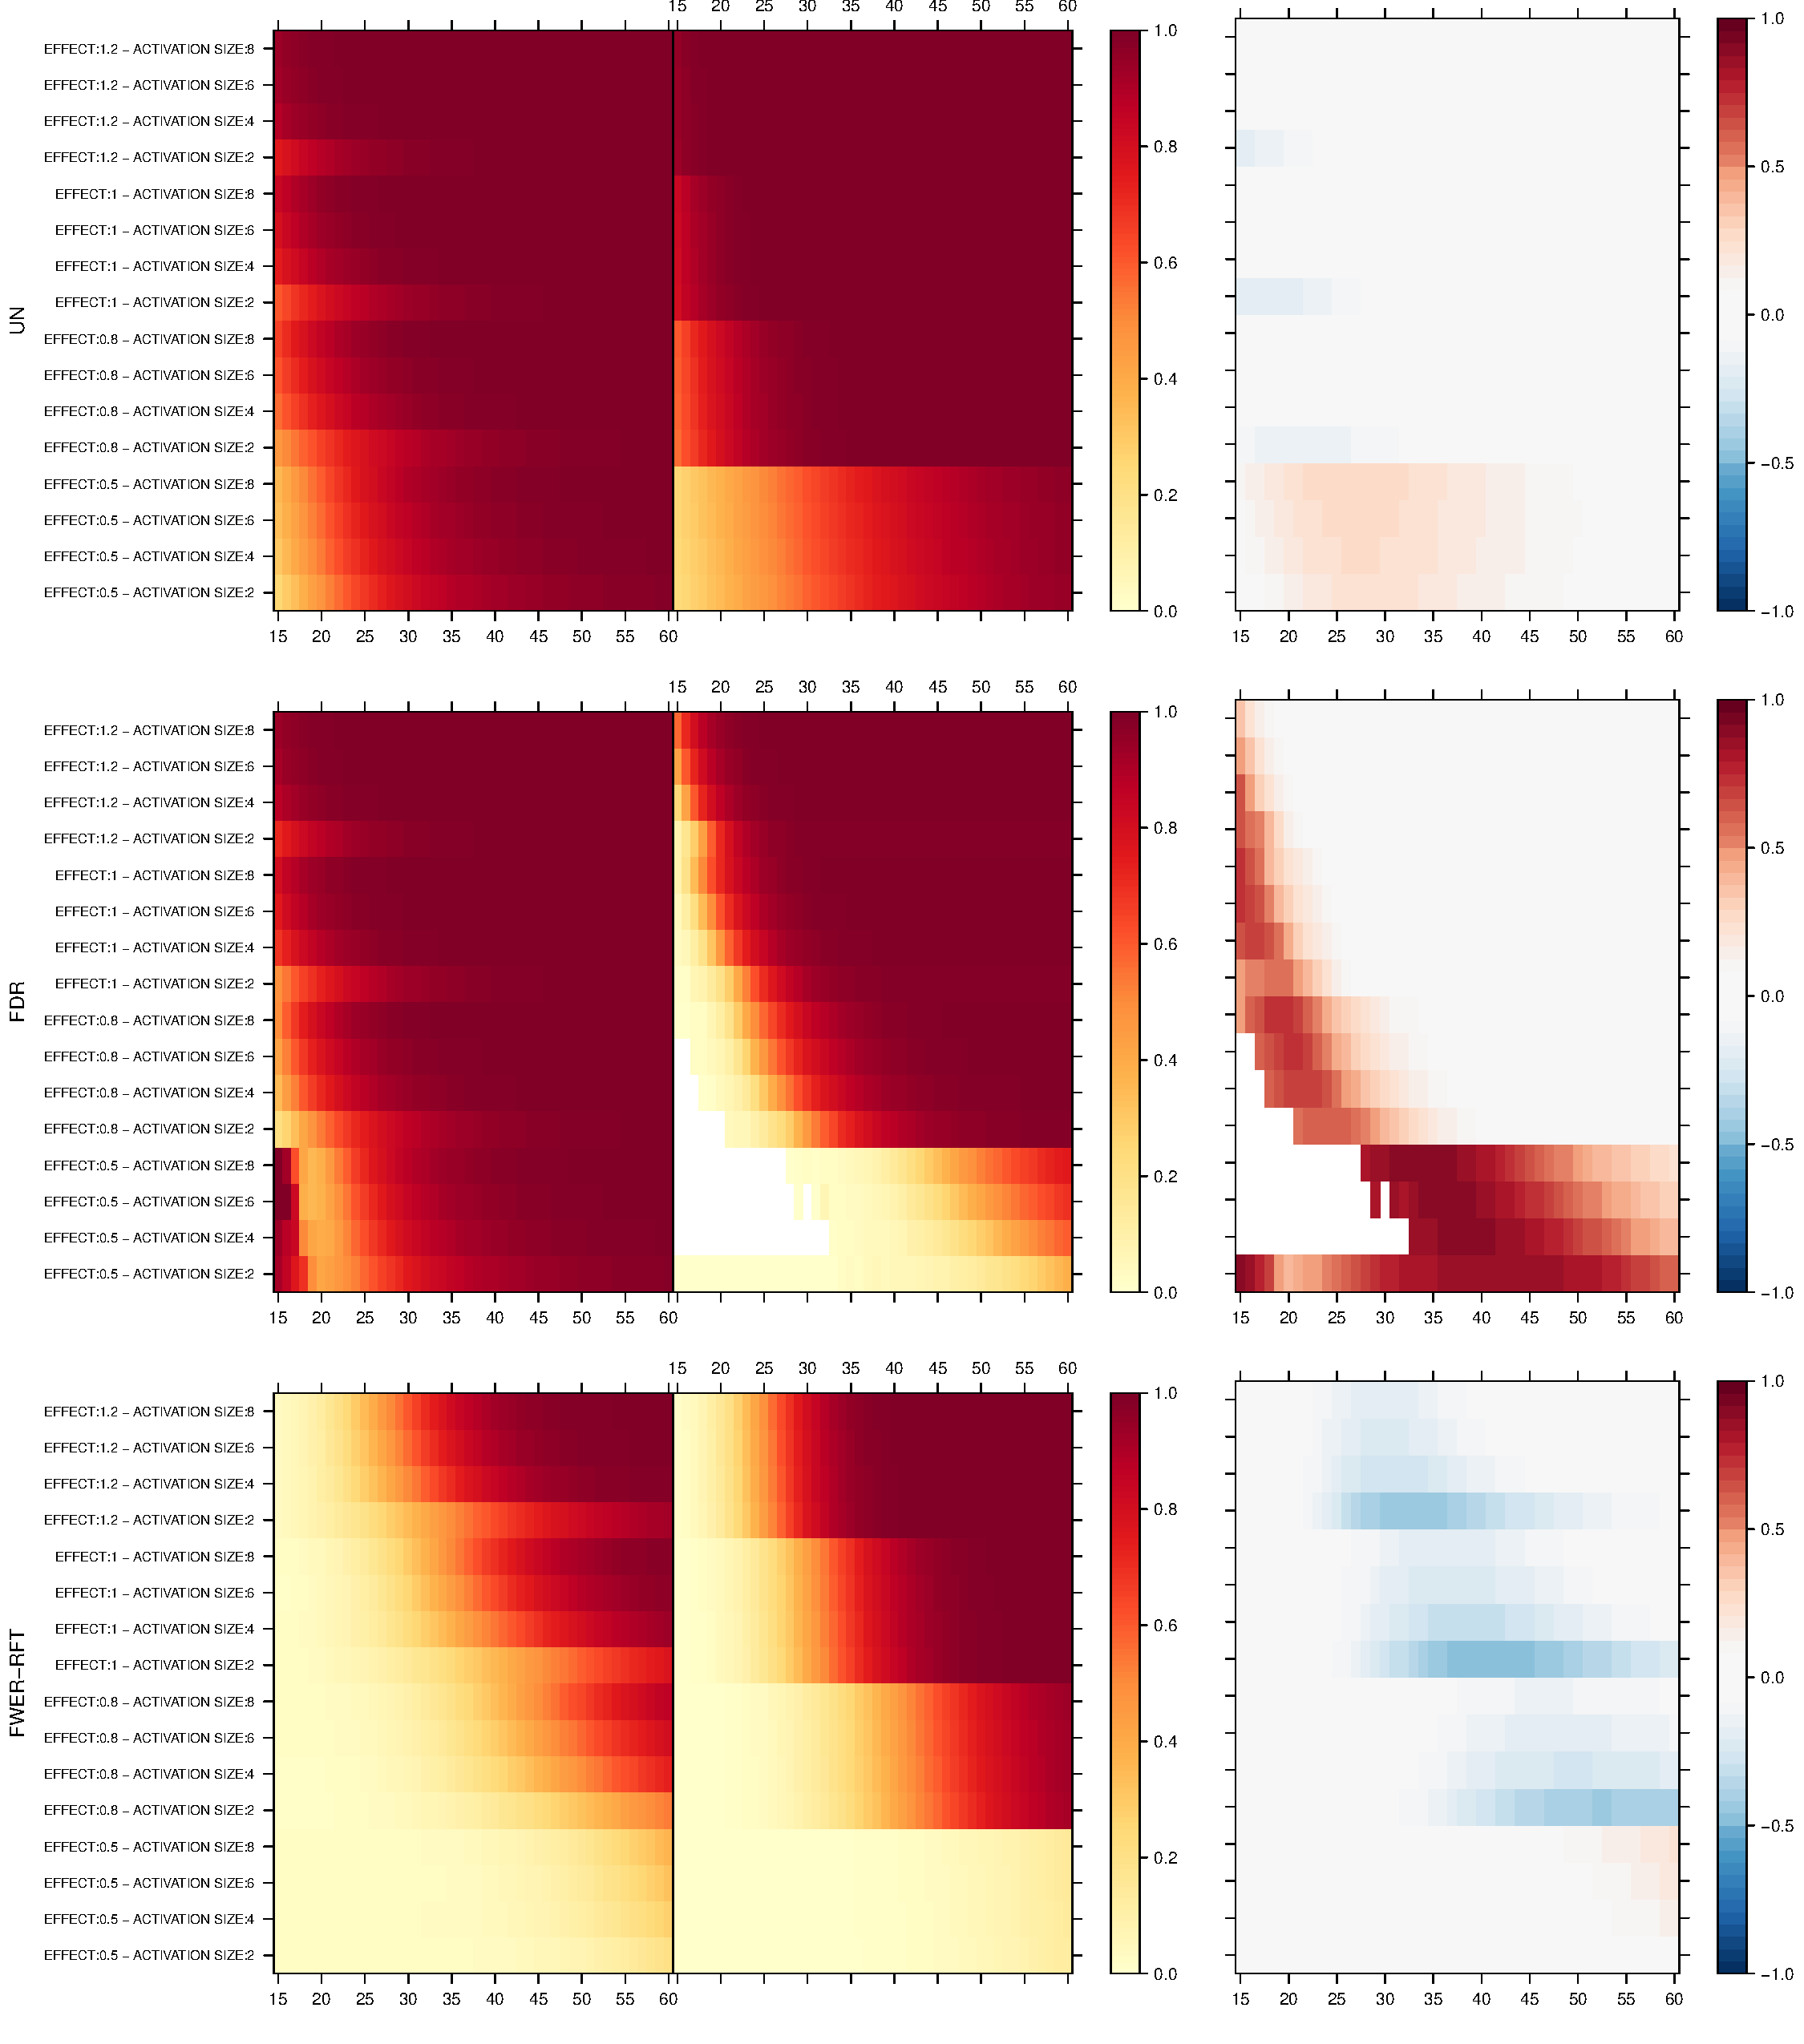
\includegraphics[scale=0.25]{figures/FIG_SIM_power_15_NOMASK_3_0.pdf}
\caption{Plots of the peakwise average power with error rate control at 5\% for different effect sizes and different amounts of activation, when using a screening threshold at 3.0.}
\end{figure}
\end{center}


\begin{center}
\begin{figure}[h]
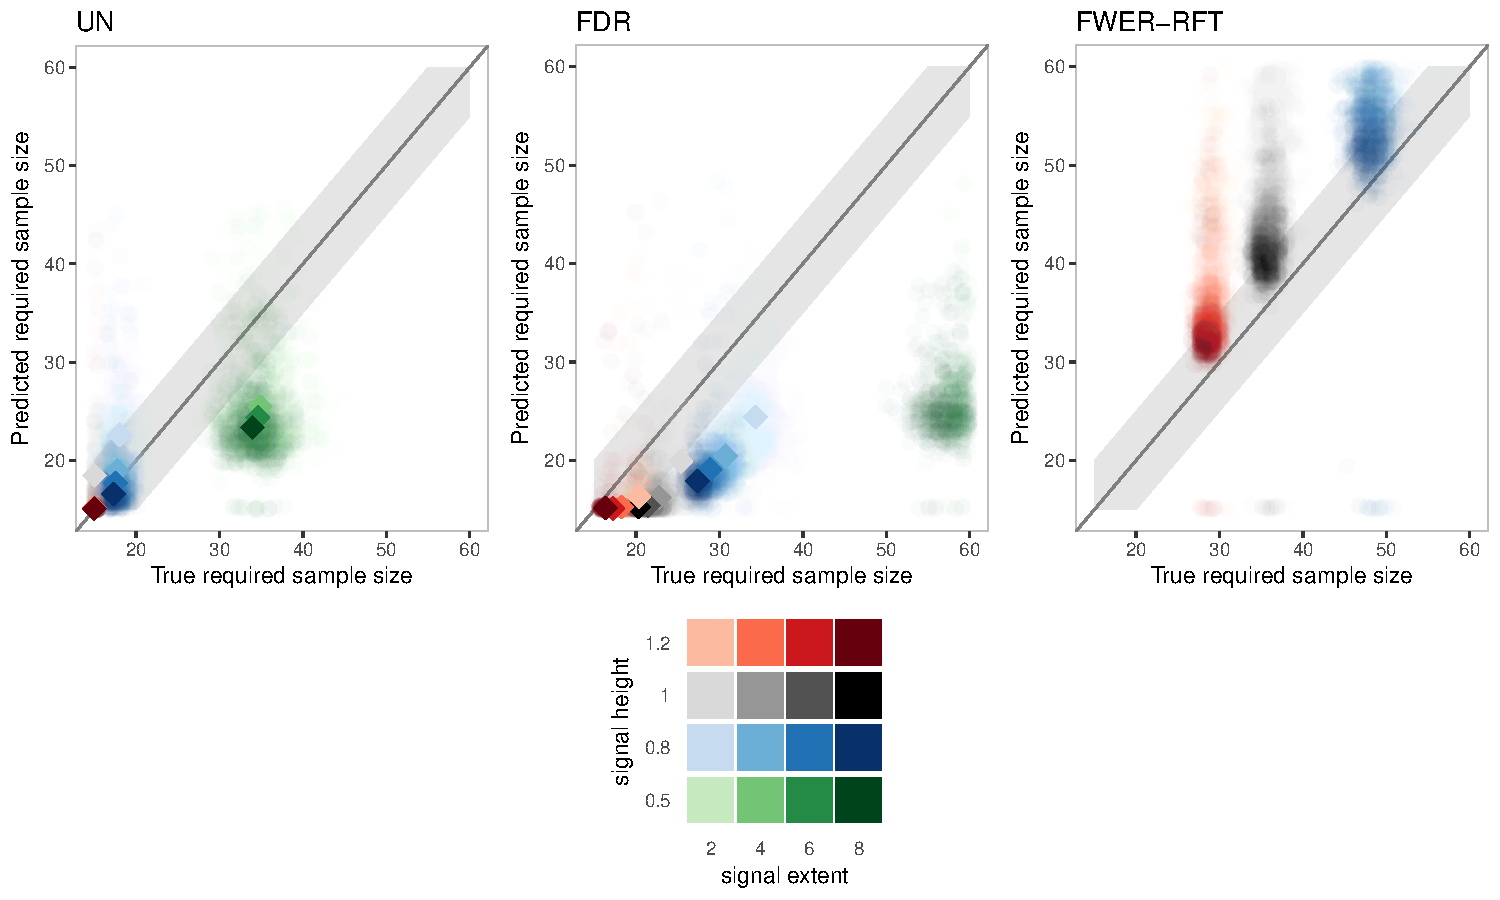
\includegraphics[scale=0.35]{figures/FIG_SIM_sscalc_15_NOMASK_3_0.pdf}
\caption{Plots of the predicted and true required sample size when 80\% power is desired. The different plots refer to the different multiple testing procedures, when using a screening threshold at 3.0.}
\end{figure}
\end{center}

\clearpage
